\chapter{Resultados}
A continuación se muestran los resultados obtenidos de la simulación presentada en la sección anterior. En general, por cada archivo de salida de datos (cada 15 minutos en este caso), se obtienen valores de velocidad, presión, temperatura, humedad, TKE, flujos superficiales, entre otras cantidades que utiliza el modelo en cada punto de la malla desplazada. Sin embargo acá no se presentan tantos datos. La muestra de datos se restringe entonces a mostrar de manera cuantitativa el comportamiento dinámico del flujo en la capa límite del dominio mas fino.
\section{Series de Tiempo}
A continuación se presentan algunos resultados representativos de las series de tiempo obtenidas con la simulación. Se muestran los datos para la magnitud de la velocidad y para la dirección del viento.

\begin{figure}[H]
	\centering
	\includegraphics[width=0.69\linewidth,page=11,trim={3cm 6cm 4cm 8cm},clip]{Imagenes/u_ts}
	%\vspace{-5mm} 
	\caption{Rapidez del viento para $\eta_l=6, z_l=123.349$ [m]}
	\label{ts_rap}
\end{figure}

\begin{figure}[H]
	\centering
	\includegraphics[width=0.77\linewidth,page=12,trim={2cm 7cm 3cm 8cm},clip]{Imagenes/u_ts}
	%\vspace{-5mm} 
	\caption{Ángulo del viento para $\eta_l=6, z_l=123.349$ [m]}
	\label{ts_ang}
\end{figure}

Es importante destacar la alta variabilidad de las variables dentro de las primeras tres horas de simulación. Esto se deben al \emph{spin-up} del modelo. La turbulencia tarda su tiempo en poder desarrollarse y por lo tanto los valores obtenidos en este rango de tiempo se omiten para los futuros resultados ya que contaminan la solución.
\section{Campos de Velocidad}
A continuación se presentan las figuras obtenidas para la velocidad con los datos resultados de la simulación. Se hace énfasis en dos análisis: la rapidez del viento cercano a la superficie, que permite describir la interacción con el terreno complejo, y los promedios de velocidad horizontal en los niveles verticales mas cercanos a la superficie que exhiben el potencial eólico de cada elemento de la malla.
\subsection{Rapidez Instantánea a 10 [m]}
De los resultados de la velocidad, se interpola a través de la ley logarítmica para encontrar la magnitud de la velocidad a 10 [m] sobre la superficie. Las figuras siguientes permiten caracterizar el comportamiento del aire en el terreno complejo, identificando zonas de recirculación.
\newcommand{\velins}[2]{
	\begin{figure}[H]
		\centering
		\includegraphics[width=0.69\linewidth,page=#1,trim={2cm 5cm 1cm 4.5cm},clip]{Imagenes/rapidez_ins_10m}
		%\vspace{-5mm} 
		\caption{Rapidez horizontal a 10 [m] simulada a las #2}
		\label{rap_10m_#2}
	\end{figure}
}
\velins{1}{12:00:00}
\velins{2}{12:15:00}
\velins{3}{12:30:00}
\velins{4}{12:45:00}%
\velins{5}{13:00:00}
\velins{6}{13:15:00}
\velins{7}{13:30:00}
\velins{8}{13:45:00}%
\velins{9}{14:00:00}
\velins{10}{14:15:00}
\velins{11}{14:30:00}
\velins{12}{14:45:00}%
\velins{13}{15:00:00}
\velins{14}{15:15:00}
\velins{15}{15:30:00}
\velins{16}{15:45:00}%
\velins{17}{16:00:00}
\velins{18}{16:15:00}
\velins{19}{16:30:00}
\velins{20}{16:45:00}%
\velins{21}{17:00:00}
\velins{22}{17:15:00}
\velins{23}{17:30:00}
\velins{24}{17:45:00}%
\velins{25}{17:00:00}
\velins{26}{18:15:00}
\velins{27}{18:30:00}
\velins{28}{18:45:00}%
\velins{29}{18:00:00}
\velins{30}{19:15:00}
\velins{31}{19:30:00}
\velins{32}{19:45:00}%
\velins{33}{19:00:00}
\velins{34}{20:15:00}
\velins{35}{20:30:00}
\velins{36}{20:45:00}%
\velins{37}{21:00:00}
\subsection{Velocidad Media}
Se promedian temporalmente los valores obtenidos en cada punto de malla, en cada nivel de la coordenada vertical.

A continuación se presentan los resultados para los primeros 10 niveles (relevantes para aplicaciones eólicas) y se detalla la altura media en metros a la cual se realizó la simulación.
\newcommand{\velmed}[2]{
	\begin{figure}[H]
		\centering
		\includegraphics[width=0.69\linewidth,page=#1,trim={2cm 5cm 1cm 4.5cm},clip]{Imagenes/rapidez_media}
		%\vspace{-5mm} 
		\caption{Rapidez media $\eta_l = #1$. $z_l = #2$ [m]}
		\label{rap_med_#1}
	\end{figure}
}
\velmed{1}{8.20464}
\velmed{2}{24.6166}
\velmed{3}{38.9816}
\velmed{4}{51.2991}
\velmed{5}{82.144}
\velmed{6}{123.349}
\velmed{7}{164.752}
\velmed{8}{218.859}
\velmed{9}{277.528}
\velmed{10}{345.167}
\section{Perfiles de Velocidad}
Las siguiente figuras muestran el perfil de viento medio para las cuatro ubicaciones mencionadas anteriormente.

\newcommand{\velprofile}[2]{
	\begin{figure}[H]
		\centering
		\includegraphics[width=0.7\linewidth,page=#1,trim={2cm 6cm 2cm 7.6cm},clip]{Imagenes/perfil_medio}
		%\vspace{-5mm} 
		\caption{Perfil de viento para #2.}
		\label{rap_perfil_#1}
	\end{figure}
}
\velprofile{1}{(-33.103,-71.716)}
\velprofile{3}{(-33.115,-71.708)}
\velprofile{5}{(-33.110,-71.730)}
\velprofile{7}{(-33.104,-71.704)}
\section{Espectro de Energía}
Para cada serie de tiempo obtenida en el punto de monitoreo, se realiza un análisis espectral a modo de revisar su distribución en el espacio de frecuencias.

Si bien en LES es necesario descomponer en el espacio de números de onda la señal de velocidad, se puede hacer la analogía con el espacio de frecuencias usando la hipótesis de Taylor considerando una turbulencia moderada.

A continuación se presentan los espectros para los primeros 15 niveles de la coordenada vertical. Como referencia también se grafica la ley de los $-5/3$.
\newcommand{\spectrafig}[1]{
\begin{figure}[H]
	\centering
	\includegraphics[width=0.66\linewidth,page=#1,trim={0cm 0cm 0cm 1.4cm},clip]{Imagenes/spectra}
	\vspace{-5mm} 
	\caption{Espectro de velocidad horizontal para $\eta_l = #1$}
	\label{spectra_#1}
\end{figure}
}
\spectrafig{1}
\spectrafig{2}
\spectrafig{3}
\spectrafig{4}
\spectrafig{5}
\spectrafig{6}
\spectrafig{7}
\spectrafig{8}
\spectrafig{9}
\spectrafig{10}
\spectrafig{11}
\spectrafig{12}
\spectrafig{13}
\spectrafig{14}
\spectrafig{15}



\chapter{Análisis y Conclusiones}
Del análisis de los resultados obtenidos se extraen la siguientes conclusiones:
\begin{itemize*}
	\item Debido a la simulación lograda con las bases de datos de alta resolución y aplicando LES para la turbulencia, se puede ver claramente el comportamiento del flujo sobre el terreno complejo de Punta Curaumilla. El explorador eólico reconoce toda la zona como una zona de alto potencial eólico, sin embargo, un mejor análisis permite ver la formación de zonas de recirculación y las zonas localizadas de vientos horizontales fuertes.
	\item Con respecto a los perfiles de velocidad, esto cumplen lo esperado en su forma. Como el día es de Enero, no se espera tener perfiles con formas fuera de lo común, sin embargo la comparación entre los 4 puntos permite comprobar las estadísticas obtenidas en los otros resultados.
	\item Los valores medios obtenidos para cada nivel permiten el reconocimiento de dos zonas que destacan por su alto potencial eólico y que vendrían a ser buenos candidatos para futuros proyectos eólicos. Una de estas es la costa central del dominio y la otra es la zona aguasabajo de la colina simulada.
	\item El espectro de energía obtenido de las mediciones continuas para la velocidad horizontal tiene una forma concordante con la teoría. Si bien la zona inercial no cumple a cabalidad la ley de los -5/3, esto es de esperar debido a que la turbulencia en la capa límite atmosférica está lejos de ser homogénea e isotrópica. Se puede apreciar que a medida que se aumenta en los niveles de la coordenada vertical, el espectro poco a poco va aumentando su pendiente, acercándose a los -5/3. Esto se explica debido a que lejos de la superficie ya no existen direcciones preferentes para la turbulencia y está comienza su transición a la isotropía.
\end{itemize*}
\section{Trabajo Futuro}
Para el caso de estudio revisado en este informe y su respectiva simulación queda por realizar las siguientes tareas:
\begin{itemize*}
	\item Expandir las simulaciones a una mayor ventana temporal, utilizando un mejor recurso computacional para aprovechar la paralelización del código y así obtener mejores estadísticos de la zona.
	\item Hacer un análisis de sensibilidad a los distintos factores externos de la simulación: condiciones de borde, esquemas de parametrización de la microfísica, cambiar modelos de advección-difusión, etc.
	\item Simular utilizando un dominio computacional mas grande, es decir, aumentar el número de nodos en la dirección horizontal, para que de esta forma sea representativo realizar un análisis espectral en el espacio de números de onda y obtener directamente el espectro de energía turbulenta.
	\item La utilización y comparación con otros modelos de submalla. Específicamente revisar el comportamiento con un modelo de Smagorinsky 3D y otros modelos anisotrópicos.
	\item Validar las simulaciones realizadas con mediciones reales. Estas se esperan que estén operativas en algún momento año 2018.
\end{itemize*}